\setcounter{chapter}{2}
\chapter{\tenchuongiii}
\section{Tổng quan hệ thống}
Hệ thống chương trình thử nghiệm Phần mềm chuẩn đoán bệnh lao được thiết kế theo kiến trúc Client/Server năm tầng (hình \ref{fig:client_server_ntang}), trong đó:
\begin{itemize}
	\item {\bf Tầng thứ nhất} là tầng giao diện người phân loại, cụ thể là ứng dụng client trên trình duyệt, quản lý tương tác người phân loại với ứng dụng như chọn ảnh gửi lên server… và hiển thị kết quả phân loại do server gửi về.
	\item {\bf Tầng thứ hai} là tầng server quản lý cấu hình hệ thống, ví dụ cấu hình giao thức gửi/nhận dữ liệu với client, cụ thể giao thức được sử dụng trong hệ thống là giao thức HTTP.
	\item {\bf Tầng thứ ba} là tầng server thực hiện logic xử lý các yêu cầu từ client, như	quản lý và phân phối các luồng xử lý độc lập, đảm bảo hiệu năng và chất lượng tính toán phân loại cho nhiều client trong cùng một thời điểm.
	\item {\bf Tầng thứ tư} là tầng đảm nhiệm xây dựng, tinh chỉnh và quản lý các phiên	bản mô hình phân loại cho hệ thống, với bộ ảnh huấn luyện được lấy từ tầng quản lý dữ liệu bên dưới.
	\item {\bf Tầng cuối cùng} là tầng quản lý dữ liệu, bao gồm CSDL ảnh phục vụ cho việc huấn luyện mô hình, CSDL ảnh đã xử lý từ các client nhằm mục đích bổ sung sự	đa dạng của CSDL ảnh và cải thiện độ chính xác của mô hình phân loại. Các bộ ảnh trên được lưu tách biệt để thuận tiện cho việc quản lý và đánh giá độ chính xác của các
	phiên bản mô hình huấn luyện cũng như mức độ ảnh hưởng của bộ ảnh huấn luyện lên chất lượng mô hình.
\end{itemize}
\begin{figure}[H]
	\centering
	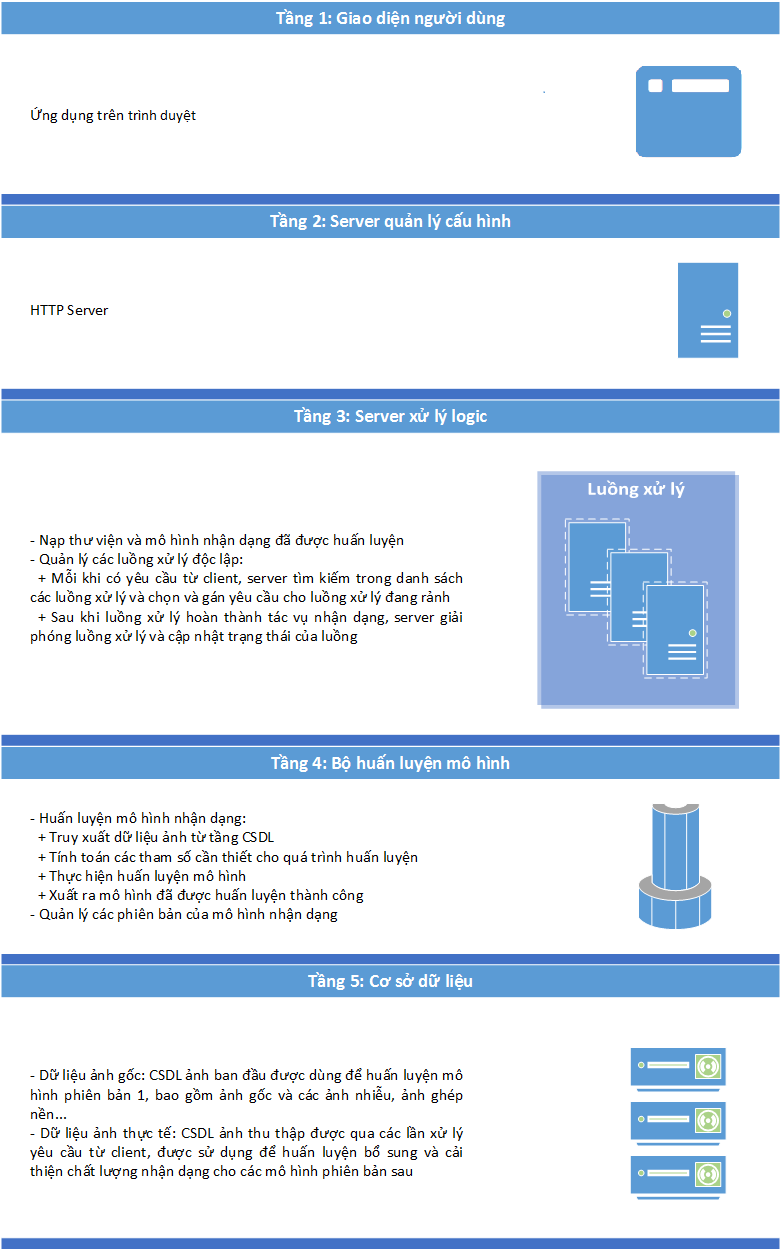
\includegraphics[width=0.8\linewidth]{images/client_server_ntang}
	\caption{Kiến trúc Client/Server n tầng.}
	\label{fig:client_server_ntang}
\end{figure}

Luồng hoạt động chính của hệ thống được thể hiện trong hình \ref{fig:app_sequence}, trong đó các bước thực hiện của server và client từ lúc khởi động ban đầu tới lúc kết thúc như sau:
\begin{itemize}
	\item Client (ứng dụng trên trình duyệt)
		\begin{enumerate}
			\item Người phân loại khởi động ứng dụng/website.
			\item Người phân loại thực hiện chọn ảnh chụp x-quang trước đó được lưu trong máy tính để gửi.
			\item Ảnh chụp được mã hóa, nén lại và gửi tới máy chủ.
			\item Ứng dụng đợi nhận kết quả phân loại từ máy chủ gửi về và hiển thị cho người phân loại
		\end{enumerate}
	\item Chương trình Server
		\begin{enumerate}
			\item Chương trình được khởi động và nạp các thư viện cần thiết.
			\item Chương trình nạp mô hình phân loại đã được huấn luyện trước đó.
			\item Giao thức gửi, nhận dữ liệu giữa ứng dụng phía client và chương trình server được cấu hình.
			\item Một loại các luồng xử lý được khởi tạo, đặt trạng thái ban đầu là trạng thái sẵn sàng.
			\item Khi có ứng dụng client kết nối tới, chương trình kiểm tra trong danh sách các luồng xử lý và chọn một luồng đang ở trạng thái sẵn sàng để nhận và tính toán dữ liệu do client gửi tới.
			\item Trong luồng xử lý:
				\begin{itemize}
					\item Bắt đầu quá trình tính toán phân loại, cờ trạng thái là “bận”.
					\item Thực hiện giải nén dữ liệu thành dữ liệu ảnh gốc.
					\item Sử dụng mô hình đã nạp để phân loại ảnh.
					\item Trả kết quả phân loại về cho ứng dụng client.
					\item Kết thúc quá trình tính toán.
				\end{itemize}
			\item Khi luồng xử lý đã hoàn thành quá trình tính toán phân loại, chương trình giải phóng luồng xử lý bằng cách cập nhật lại trạng thái hiện tại của luồng.
		\end{enumerate}
\end{itemize}
\begin{figure}[H]
	\centering
	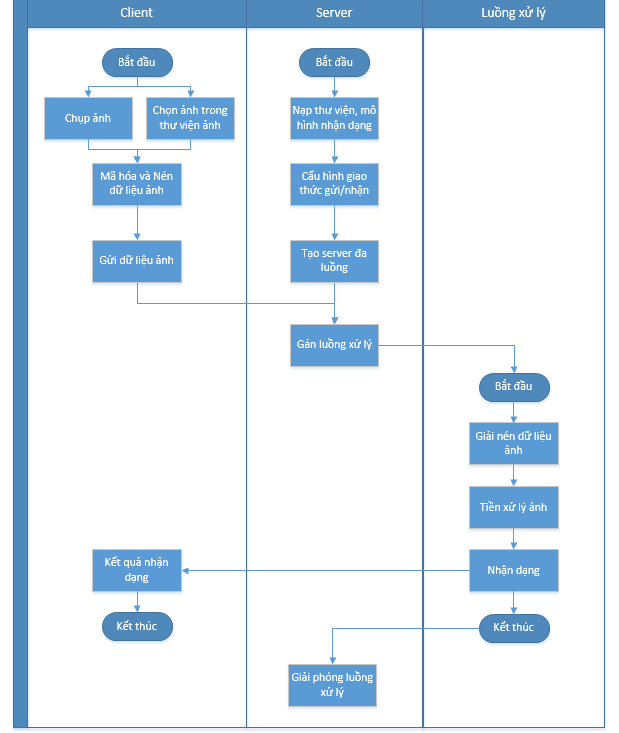
\includegraphics[width=0.88\linewidth]{images/app_sequence}
	\caption{Luồng hoạt động chính của hệ thống.}
	\label{fig:app_sequence}
\end{figure}

%\section{Kết quả thử nghiệm}

%\section{Đánh giá}